\documentclass[12pt]{scrartcl} %KOMA Klasse, Artikel
\usepackage[utf8]{inputenc}
\usepackage[T1]{fontenc}
\usepackage[ngerman, english]{babel}
\usepackage{lmodern}
\usepackage{graphicx}
\usepackage{float}
\usepackage{booktabs}
\usepackage[detect-all,exponent-product=\cdot , decimalsymbol=.]{siunitx}
\usepackage{hyperref}
\hypersetup{colorlinks,linkcolor=black,urlcolor=blue, citecolor=black}
\usepackage{subcaption}
\usepackage{listings}
\usepackage{color}
\usepackage[automark]{scrpage2}
\usepackage{setspace}
\onehalfspacing

\usepackage[figurename=Fig.,tablename=Tab.]{caption}

\pagestyle{scrheadings}
\clearscrheadfoot
\ohead{Miguel Steiner}
\ihead{\headmark}
\ifoot{FEBISS Manual}
\title{Free Energy Based Identification of Solvation Sites}
\ofoot{\pagemark}
\setheadsepline[\textwidth]{1pt}
\setfootsepline[\textwidth]{1pt}
\subject{FEBISS Manual}
\subtitle{}
\author{author: Miguel Steiner\\maintainer: Maren Podewitz (maren.podewitz@uibk.ac.at)}
\date{}
\newlength{\minuslength}
\settowidth{\minuslength}{--}


\begin{document}


\maketitle
\newpage


\newpage
\section{Installation}

FEBISS requires a Linux system and Python3. It can be installed using pip (pip3) once the repository has been cloned:
\begin{lstlisting}[language=bash]
$ git clone https://github.com/PodewitzLab/FEBISS
$ pip install ./febiss
\end{lstlisting}
or directly via PyPi
\begin{lstlisting}[language=bash]
$ pip install febiss
\end{lstlisting}
A non super user can install the package using a virtual environment, or the --user flag.

\subsection{Basic Requirements}
FEBISS is expected to run on Linux systems and the following programs/packages are required:
\begin{itemize}
\item Python3
\item Git
\item GCC >= v7.0.0
\item FEBISS Python Package
\end{itemize}
The main Python package called FEBISS requires only basic additional packages, which will be automatically installed when installing FEBISS, using pip. These packages are:
\begin{itemize}
	\item matplotlib
	\item numpy
	\item pyyaml
	\item scipy
\end{itemize}

\subsection{C++ Requirements}
To run analyses of trajectories the open-source software CPPTRAJ modified with the GIGIST repository is used. These dependencies are not necessary for the installation of FEBISS, but rather FEBISS provides a script to set-up these dependencies via
\begin{lstlisting}[language=bash]
$ febiss_setup
\end{lstlisting}
This will show you a help message with all necessary details. If you already have a sufficiently modified CPPTRAJ version, you can simply write the path to the binary in the .febissrc.yaml file in your home directory:
\begin{lstlisting}[language=bash]
CPPTRAJ_BIN: /path/to/binary
\end{lstlisting}
Otherwise call the \textit{febiss\_setup} script with the yaml file with your desired CPPTRAJ configuration or call
\begin{lstlisting}[language=bash]
$ febiss_setup default
\end{lstlisting}
for both openmp and cuda supported CPPTRAJ in the~.dependencies\_febiss directory in your home. If the setup was successful, you are now able to analyze trajectories with the program.\\
Please be aware that CPPTRAJ may require libraries that cannot be installed via FEBISS, but have to be installed by the user first. CPPTRAJ makes use of the following libraries:
\begin{itemize}
\item NetCDF
\item BLAS
\item LAPACK
\item Gzip
\item Bzip2
\item Parallel NetCDF (-mpi build only, for NetCDF trajectory output in parallel)
\item CUDA (-cuda build only)
\item FFTW (mostly optional; required for PME functionality and very large FFTs)
\end{itemize}
We therefore recommend to first install some basic libraries via
\begin{lstlisting}[language=bash]
$ sudo apt-get install libblas-dev liblapack-dev libbz2-dev
$ sudo apt-get install libnetcdf-dev
\end{lstlisting}
Should you encounter difficulties in the installation of CPPTRAJ, we refer to the README of the GIGIST and CPPTRAJ repositories.

\section{Inputs for analysis}
The analysis is performed with the command line program febiss. It expects exactly one command line argument, which is a link to a yaml file containing all settings. To get a template yaml file with all settings, you can simply call
\begin{lstlisting}[language=bash]
$ febiss_settings
\end{lstlisting}
This will write a settings file called \textit{all-settings.yaml} in your current directory. If you open it, you will notice that you need to fill out two fields for the program to work. You have to give the full filename to the topology file and the basename of your trajectory file(s) without the file format ending, which is specified in a different field. If you filled these out correctly, you can call
\begin{lstlisting}[language=bash]
$ febiss all-settings.yaml
\end{lstlisting}
to start the analysis. Depending on the number of frames, this analysis might take a few minutes. Afterwards, the graphical user interface (GUI) in form of a bar plot should appear.

\section{Description of all settings}
The easiest way of writing your settings file is to first execute the \textit{febiss\_settings} script as mentioned above. The yaml file is split in two major blocks. The gist block includes all possible settings linked to the execution of CPPTRAJ. These options are:
\begin{itemize}
	\item trajectory\_name: Has to be filled out, only include the basename of the trajectory file(s)
	\item top: Has to be filled out, full name of the topology file including file format suffix
	\item cpptraj\_command\_file: Filename where all CPPTRAJ commands are written in
	\item frame\_selection: Give a selection of frames as string in identical syntax as in CPPTRAJ. We recommend to include as many frames as possible, but this will increase the time of analysis
	\item gist\_grid\_file: Filename, where the grid of the GIST analysis is written into. The grid is represented as H nuclei. This serves the purpose to check if your GIST grid is sufficient if you have a large solute
	\item gist\_out\_file: Filename, where the usual GIST output is written into
	\item grid\_center: The Cartesian coordinates of the GIST grid center, if None is given, the GIST default, the origin, is used. Please be aware that your solute residues are automatically centered at the origin
	\item grid\_lengths: The number of voxels along each Cartesian axis, it can be given either as a single number for cubic grids or as three numbers for rectangular grids
	\item grid\_spacing: The distance between neighboring voxels of the GIST grid in \si{\angstrom}.
	\item rdf: Whether a RDF analysis should be performed
	\item rdf\_names: A dictionary with the element symbols or CPPTRAJ command as key and the name of the file as value. If you change something here, please also change the option with the same name in the plotting block. The backslashes in 'center of solute' are necessary for CPPTRAJ file write out, but are not necessary in the dictionary in the plotting block.
	\item refdens: The reference density of the water model. The default corresponds to the value of TIP3P
	\item solute\_residues: The CPPTRAJ command to define your solute. The default :1 corresponds to residue number one.
	\item trajectory\_format: The format suffix of your trajectory file(s). The applied command to read in your trajectory is trajin [trajectory\_name]*[trajectory\_format]
	\item water\_angle: The ideal angle of your water model. The default is 104.57
\end{itemize}
The plotting block handles all settings related to the analysis of the CPPTRAJ output and the GUI. The options cutoff1, cutoff2, and displayed\_waters can also be changed later, if no water is selected. Please be aware that the distance categorization of FEBISS deliberately ignores apolar hydrogens. This allows to easier distinguish between water molecules close to hydrophilic and hydrophobic regions of the solute with the default cutoff of \SI{3}{\angstrom}.\\
All options for plotting are:
\begin{itemize}
	\item colors: A dictionary containing the different colors in the plot as hex strings. Do	not change the keys, but only the values, if you prefer different colors.
	\item cutoff1: The first cutoff in the bar chart
	\item cutoff2: The second cutoff in the bar chart
	\item display\_once: Whether the program should ask you for a change of the cutoffs	and displayed waters if you did not select any water
	\item displayed\_waters: The number of displayed waters in the bar chart. Either enter a number or 'all'
	\item dpi: The dpi of the displayed and saved images
	\item febiss\_file: The name of the file, which contains the solute and all FEBISS waters.
	\item fontsize: The fontsize in the bar chart
	\item height: The height of the GUI window
	\item marks: X-coordinates of vertical dotted lines to mark certain number of water molecules
	\item number\_xtics: The number of tics on the x-axis in the bar chart
	\item orientation: The orientation of the GUI window
	\item plotname: Filename of the saved bar chart
	\item rdf\_names: See in gist block
	\item selected\_plotname: Filename of the saved bar chart including the selected bars
	\item testing: Internal testing flag
	\item transparent: Whether the saved plot should be transparent or not
	\item width: The width of the GUI window
	\item xlabel: The label of the x-axis of the bar chart
	\item y\_numbers: The value difference between labeled tics on the y-axis
	\item ylabel: The label of the y-axis of the bar chart
\end{itemize}

\section{Graphical user interface}
After the CPPTRAJ analysis, a GUI-like matplotlib window should open. There, you
see the water molecules ranked lowest in free energy represented as bars and colored according to the distance criteria. In order to select water molecules to obtain the microsolvated structure, simply click on the individual bars, which should then turn green or your selected color in the settings file. You can deselect them by clicking again. You can also plot some RDFs with the button on the top right to help you with your decision. The RDFs are scanned for local maxima and minima and integral values are displayed on hovering the mouse over them.\\
If you are not happy with the distance thresholds or the number of water molecules, simply close the window with \textbf{no} waters selected. You will be asked, whether you want to change the thresholds and what the new thresholds should be. Then, the window should reappear.\\
If you close the window \textbf{with} waters selected, you approve your selection and a PyMOL session with the selected microsolvated structure will appear, if PyMOL is installed on your system.

\section{Flowchart}
\begin{figure}[H]
	\centering
	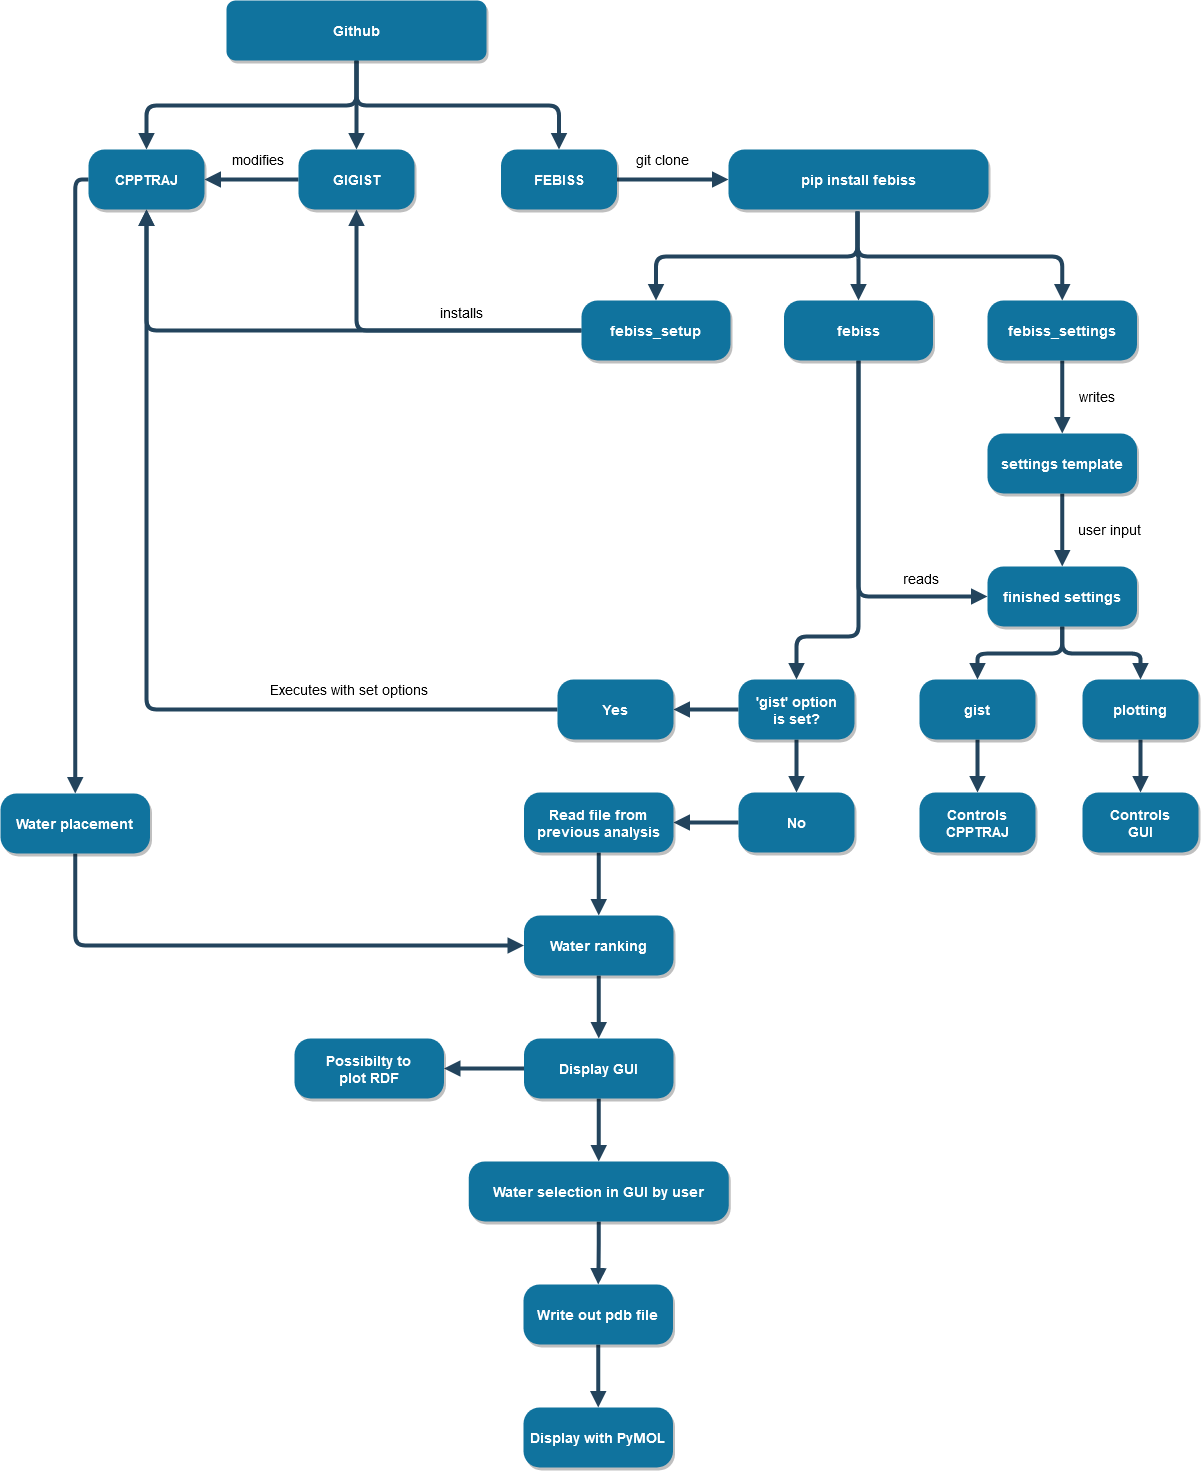
\includegraphics[width=\linewidth]{flowchart.png}
	\caption{Flowchart of the Python package and its C++ dependencies.}
\end{figure}

\end{document}